\documentclass{article}
\usepackage{tikz} 

\usepackage{forest}
\begin{document}
\section*{exercice01}
    \subsection*{a) les sources du problème d’apprentissage}
    \begin{enumerate}
        \item La premi`ere correspond au nombre de cycles durant lesquels la perfor-
        mance de l’agent reste sous-optimale pour la tˆache de d ́ecision donnee.
        \item La seconde correspond aux ressources de calcul n ́ecessaires durant chaque
        cycle `a l’agent pour r ́eviser sa strat ́egie et choisir une action.



    \end{enumerate}
    \subsection*{b) une d ́efinition du modéle d’apprentissage}
    mod`ele d’apprentissage est un cadre formel donnant une mesure de ces deux
    sources de complexit ́e. Les observations, les actions et le feedback peuvent
    influer sur la difficult ́e de l’apprentissage
    \subsection*{c) Expliquer comment les observations, les actions et le feedback peuvent influer sur la difficult ́e de l’apprentissage}
    1. \underline{L’observation}:  l’espace des observations
    la dimension peut etre immense, voire infini
 les valeurs de certains attributs peuvent ˆetre impr´ecises, erron´ees, ou
encore absentes.
environnements partiellement observables alors ’une situation inceain \\
2. \underline{L’action}: les actions sont des decision soit simple ou complex,
 l’espace des d´ecisions poss`ede une structure combinatoire; les d´ecisions
peuvent prendre la forme d’arbres, de graphes, ou encore d’hypergraphes
Les actions simples peuvent avoir un impact sur la difficult´e de l’apprentissage
selon la mani`ere dont elles influent l’environnement (´episodique/s´equentiel)\\
3. \underline{Feedback}:Le type de feedback d´efinit le mode d’apprentissage



\section*{exercice2}

    \subsection*{Donner avec explication les composants du probl`eme l’apprentissage supervis ́e de porte logique XOR}
    Une fonction XOr doit renvoyer une valeur vraie si les deux entr ́ees ne sont
    pas  ́egales et une valeur fausse si elles sont  ́egales -l’espace des entr ́ees est X =(0, 1)n et l’espace des sorties est Y = 0,1.
    ’hypothèse associée à ω = (w, θ) est définie par 
    hω(x) = tanh (x)  
    le produit scalaire entre w et x et tanh(z) est la fonction qui retourne le signe du scalaire z

\section*{exercice03}
    \subsection*{x1 x2 x3 x4}

    \begin{forest}
        [x1, for tree={draw,circle}
            [x3[0][x4[0][1]]]
            [x2[x3[0][x4[0][1]]][1]]]
    \end{forest}


\section*{exercice04}
    \subsection*{a) la diff ́erence entre une requˆete d’appartenance et une
    requˆete d’ ́equivalence est}
    \begin{enumerate}
        \item Une requˆete d’appartenance (MQ) associe `a une instance x pos ́ee par
        l’apprenant la r ́eponse oui si h(x) = 1, et non sinon.
        \item Une requˆete d’ ́equivalence (EQ) associe `a une hypoth`ese h pos ́e par
        l’apprenant la r ́eponse oui si h = h, et non sinon
    \end{enumerate}
    \subsection*{b) Si pour toute instance (x1, x2, x3) quelle est l’hypoth`ese
    (le concept) le plus sp ́ecifiqu} est h1((x1,x2,x3)) = x1
    \subsection*{c) Si h(x1,x2,x3) = x1 x2 et la requˆete est h((0,1,1)) =
    0}
    \begin{enumerate}
        \item le type de cette requˆete est requˆete d’appartenance (MQ)
        \item et si h*((0,1,1)) = 1, requˆete d’ ́equivalence (EQ)
        \item Si le contre exemple est (0,1,0) mettre `a jour h. h((0,1,0)) = 1

    \end{enumerate}
\section*{exercice05}
%not solutied
\section*{exercice06}
    \subsection*{la diff ́erence entre le mod`ele agnostique et le mod`ele
    PAC}
    Dans le mod`ele “agnostique”, la distribution D est arbitraire, ce quiimplique
    qu’il n’existe a priori aucune d ́ependance fonctionnelle entre une instance x
    et une d ́ecision y dans un exemple tir ́e dans D. En revanche, dans le mod`ele
    (PAC), nous supposons qu’il existe uned ́ependance fonctionnelle gouvern ́ee
    par une fonction cible\\
    \\
    \line(144,0){5555}
\begin{center}
   \huge PAL
\end{center}

    \section*{exercice01}
    \begin{enumerate}
    \item  A[]B = B[]A $\to$ Commutativité
        \item A[]stop = stop[]A = A $\to$ Zéro absorption
    \item  A[](B[]C) = (A[]B)[]C $\to$ Associativité 
        \end{enumerate}
\section*{exercice02}
\section*{exercice03}
    \subsection*{process one [a,b,c] a; (b; stop [] c; stop) endproc}
    \begin{forest}
        [one,for tree={parent anchor=south, child anchor=north, fit=band}
        [a[b[stop]][c[stop]]]]
    \end{forest}
    \subsection*{process two [a,b,c] a; b; stop [] a; c; stop Endproc}
    \begin{forest}
        [two,for tree={parent anchor=south, child anchor=north, fit=band}
        [a[b[stop]]]
        [a[c[stop]]]]
    \end{forest}
    \subsection*{P1 := a; (b; d; stop [] c; stop)}
    \subsection*{process two [a,b,c] a; b; stop [] a; c; stop Endproc}
    \begin{forest}
        [two,for tree={parent anchor=south, child anchor=north, fit=band}
        [a[b[stop]]]
        [a[c[stop]]]]
    \end{forest}
    \subsection*{P1 := a; (b; d; stop [] c; stop)}

    \begin{forest}
        [p1,for tree={parent anchor=south, child anchor=north, fit=band}
        [a[b[d[stop]]]
        [c[stop]]]
        ] \end{forest}
    
\section*{exercice04}
    \subsection*{Ecrire des spécifications lotos pour les circuits logiques: and, or et 
    xor}
   \subsection*{AND}
    specification circuitlogiqueAND [a,b,c] :noexit \\
    type BIT is \\
        sorts BIT\\
        opns 0 (*! constructor *), \\
            1 (*! constructor *) : -> BIT\\
        and : BIT ,BIT-> BIT\\
        eqns \\
            ofsort BIT \\
            and (0,0) = 0; \\
            and (0,1) = 0; \\
            and (0,1) = 0; \\
            and (1,1) = 1; \\
    endtype\\ 
    behaviour\\ 
        gate_and[a, b, c]\\
    where \\
        process gate_AND[a, b] : noexit :=\\ 
        a ?aa:Bit; b?bb:Bit;  c!and(aa,bb); stop \\
        endproc \\
    endspec\\
    %or
    \subsection*{OR}
    specification circuitlogiqueOR [a,b,c] :noexit \\
    type BIT is \\
        sorts BIT\\
        opns 0 (*! constructor *), \\
            1 (*! constructor *) : -> BIT\\
        or : BIT ,BIT-> BIT\\
        eqns \\
            ofsort BIT \\
            or (0,0) = 0; \\
            or (0,1) = 1; \\
            or (0,1) = 1; \\
            or (1,1) = 1; \\
    endtype\\ 
    behaviour\\ 
        gate_OR[a, b, c]\\
    where \\
        process gate_OR[a, b] : noexit :=\\ 
        a ?aa:Bit; b?bb:Bit;  c!or(aa,bb); stop \\
        endproc \\
    endspec\\
  
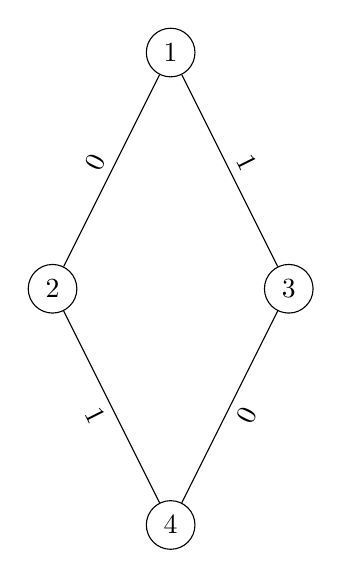
\begin{tikzpicture}[main/.style = {draw, circle}]
 
\node[main, xshift=3cm, yshift=3cm] (1) {1};
\node[main, xshift=1.5cm, yshift=0cm] (2) {2};
\node[main, xshift=4.5cm, yshift=0cm] (3){3};
\node[main,xshift=3cm, yshift=-3cm] (4) {4};
\draw (2) -- node[midway, below , sloped ] {1}(4);
\draw (2) -- node[midway, above,sloped ] {0}(1);
\draw (1) --node[midway, above,sloped ] {1} (3);
\draw (3) -- node[midway, below ,sloped ] {0}(4);


\end{tikzpicture}
    %xor
    \subsection*{XOR}
    specification circuitlogiqueXOR [a,b,c] :noexit \\
    type BIT is \\
        sorts BIT\\
        opns 0 (*! constructor *), \\
            1 (*! constructor *) : -> BIT\\
        xor : BIT ,BIT-> BIT\\
        eqns \\
            ofsort BIT \\
            xor (0,0) = 0; \\
            xor (0,1) = 1; \\
            xor (0,1) = 1; \\
            xor (1,1) = 0; \\
    endtype\\ 
    behaviour\\ 
        gate_XOR[a, b, c]\\
    where \\
        process gate_XOr[a, b] : noexit :=\\ 
        a ?aa:Bit; b?bb:Bit;  c!xor(aa,bb); stop \\
        endproc \\
    endspec\\

    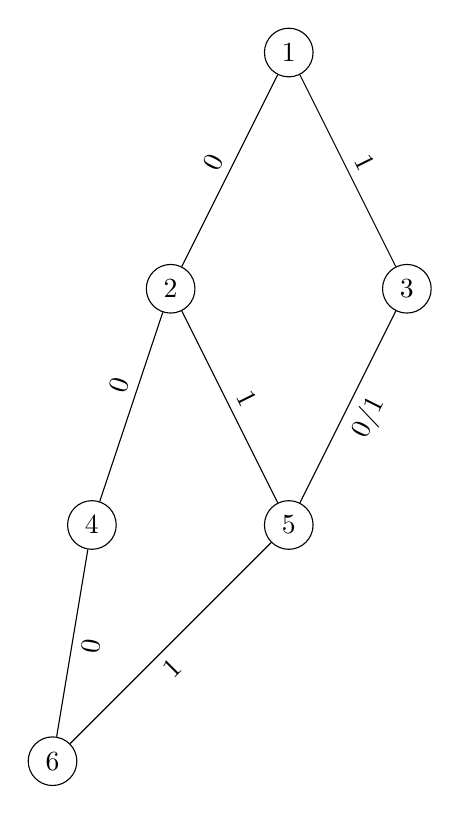
\begin{tikzpicture}[main/.style = {draw, circle}]
 
        \node[main, xshift=3cm, yshift=3cm] (1) {1};
        \node[main, xshift=1.5cm, yshift=0cm] (2) {2};
        \node[main, xshift=4.5cm, yshift=0cm] (3){3};
        \node[main,xshift=0.5cm, yshift=-3cm] (4) {4};
        \node[main,xshift=3cm, yshift=-3cm] (5) {5};
        \node[main,xshift=0cm, yshift=-6cm] (6) {6};
        
        \draw (2) -- node[midway, above , sloped ] {1}(5);
        \draw (2) -- node[midway, above,sloped ] {0}(1);
        \draw (1) --node[midway, above,sloped ] {1} (3);
        \draw (3) -- node[midway, below ,sloped ] {0/1}(5);
        \draw (2) -- node[midway, above right , sloped ] {0}(4);
        \draw (4) -- node[midway, below , sloped ] {0}(6);
        \draw (5) -- node[midway, below left, sloped ] {1}(6);
        
        \end{tikzpicture}
\end{document}

